% !TEX root = ../../thesis.tex

% Photo Yves Gellie
% \cleartoleftpage
% 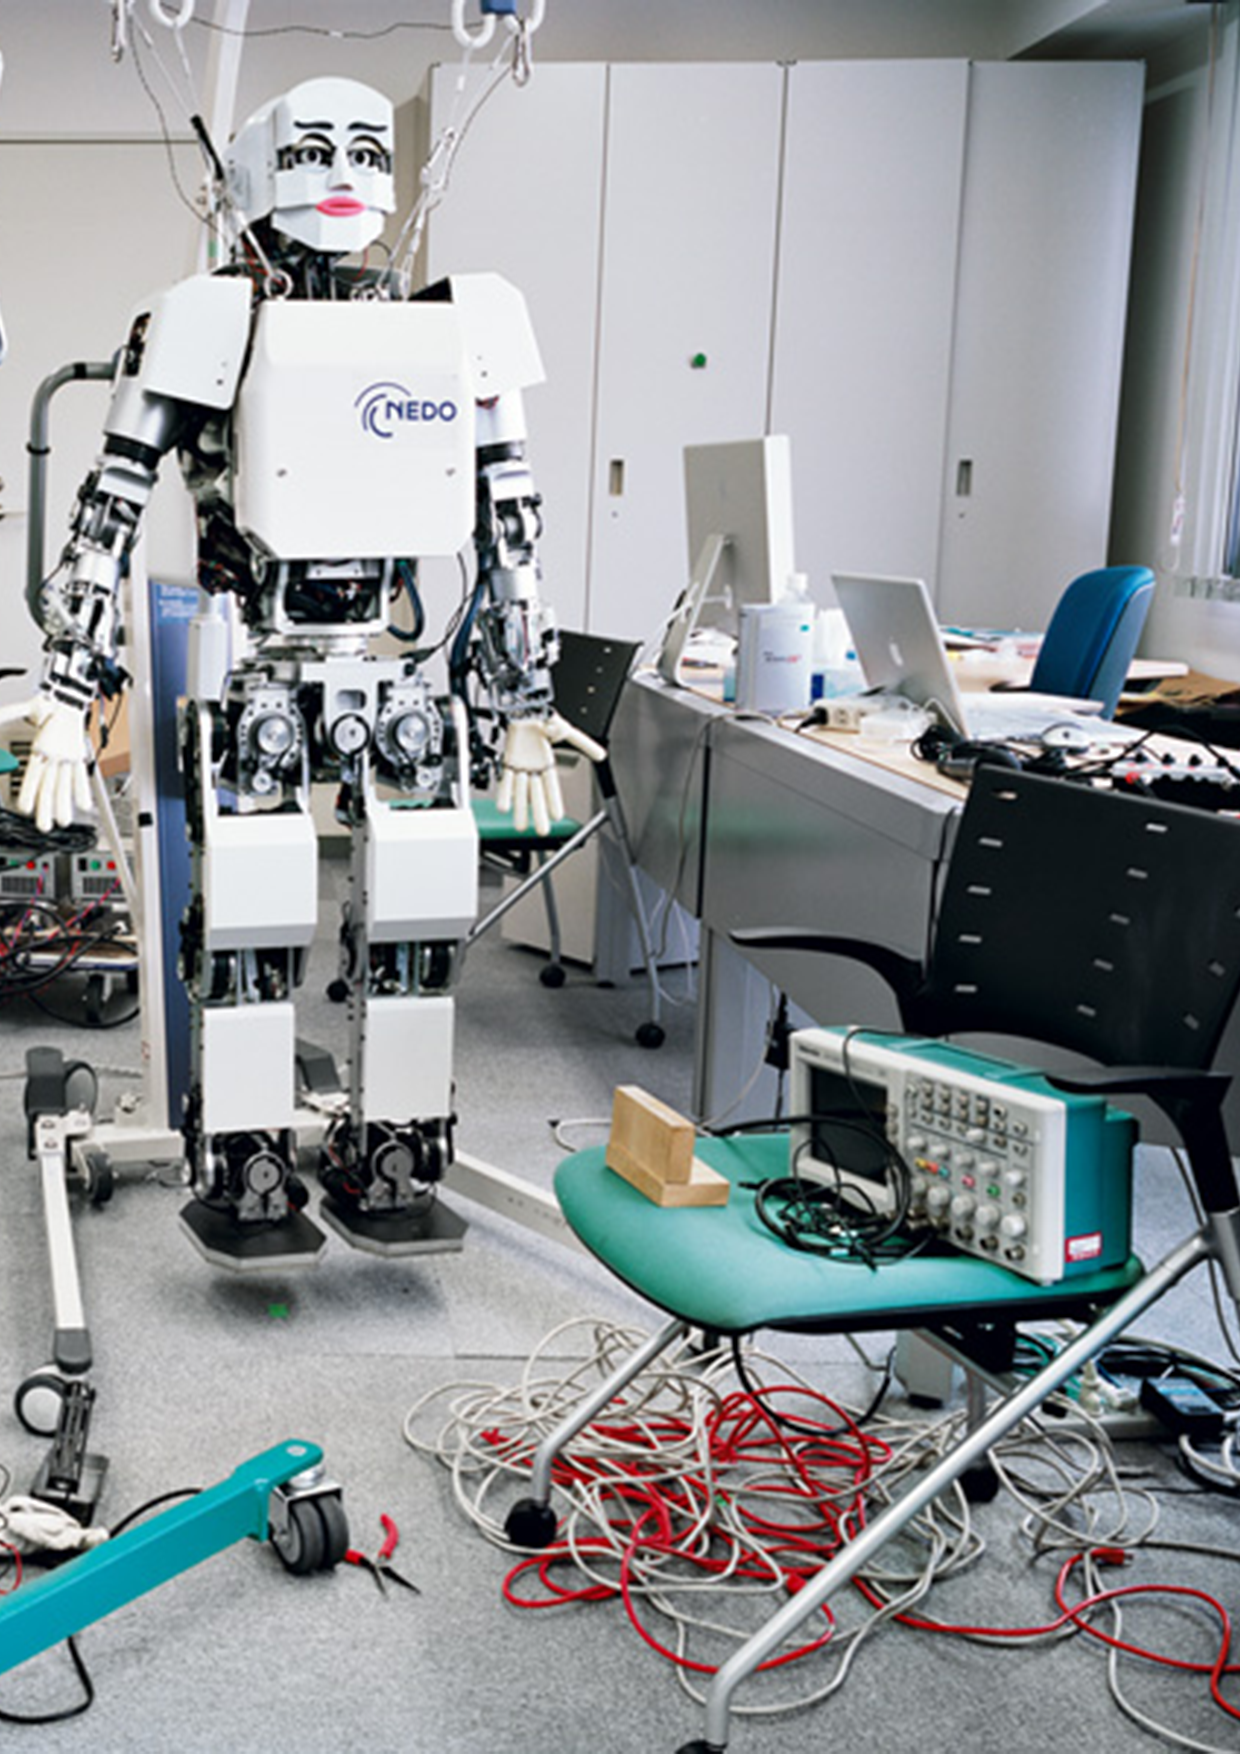
\includepdf{../media/chapter_illustration/robot_setup.pdf}
\chapter{Review of experimental methods} % (fold)
\label{cha:experimental-methods}

\cleanchapterquote{The world is its own best model.}{Rodney Brooks}


\section{Introduction} % (fold)
\label{sec:platform-introduction}

As we showed it in the previous chapter, an interesting evolution of the last decades in the robotics field is the demonstration of the importance of the robot morphology and its impact on the cognition and control while opening new horizons to achieve more adapted and robust behaviour in open-ended environment with unpredictable interaction.

However as Rodney Brooks explained, exploring interaction between morphology, cognition and environment requires real world experimentations. Indeed embodiment artificial intelligence~\parencite{Pfeifer07} needs to act in the real world to permit the emergence of complex behaviour. The real world includes a large amount of constraints such as inertia, multi-point physical contacts, friction, multi-body dynamic and impacts which are complicated to realistically model without involving considerable engineering resources. Moreover, if ones are interested by exploring robotics behaviour in an open-ended environment with human interaction, the handle the unpredictability will be limited to a small subset of cases.

From another angle, "The world is its own best model" and if we can use simulation for exploring well defined concepts, the exploration of emergent complex behaviours based on interaction between robot self-dynamics and the environment appears easier and less expensive if conducted directly in the real world.
Moreover, as Luc Steels explained~\parencite{Steels1991emergence}, the actual behaviour is emerging from the interaction between the controller, the morphology and the environment. Some could argue that adding actual morphology and ecological niche add unnecessary complexities to a problem we already have difficulty to solve by just taking care of the control. Yet it appears some behaviours cannot be achieved without the real physic complexity. Brilliant examples are the passive/semi-passive walking robots (presented in section~\ref{sub:passive_principle}). These robots are technically rather simple, just composed by a mechanical structure with proper link size and foot shape, the establishment of a model should be rather easy but their real dynamic is very difficult to simulate on a classic physical simulator. Indeed, all complex physic effects (e.g. shocks, friction, inertia) contribute to the achievement of the passive walking.

One of the best state of the art work in this domain is done by the Delft University with the different passive and semi passive walkers they built (REF). Desiring to explore biped locomotion, we had a discussion with Martijn Wisse on simulation strategy to add semi-passive abilities to Poppy. Here is his testimony when they tried to make their robot walk in simulation after managing to create the real one:

\begin{formal}

Even after obtaining a successful walking motion, we did not manage to create a simulation that walked successfully using the same controller parameters. We tried very hard with some of the best people, but we didn’t succeed. The reason was, I think, that our type of control (using the emergent behaviour of a set of simple reflex-like controllers) was highly sensitive to hardware effects like friction. Normally, one uses a local joint controller to make the joint follow a desired trajectory independent of the exact amount of friction. The local controller "abstracts these hardware effects away", if you know what I mean. This makes the behaviour of the whole system quite predictable. However, in our robots, we did not have this kind of abstraction as we were not following trajectories, and thus a little bit of extra friction has an effect on the entire motion.

We did spend a long time making a high-fidelity model in Adams, and also using other methods, but eventually we gave up without success.

\signed{Martijn Wisse - Associate professor at Delft University of Technology}
\end{formal}

Thus results obtained in simulator are difficultly transposable in a real platform and vice-versa. One of the main reason seems to be the complexity to realistically handle non-perfect components e.g. non-linear friction in joints, feet/ground reactions and so on. Yet the interesting contributions of the robot morphology on its behaviour is precisely in the aspect we have currently difficulties to model correctly.

This raised a major limitation for the results reproducibility in the scientific community. While it is rather simple to transfer experiments conducted in a simulator by sharing the software material, sharing real world experiment is way more challenging.

In this chapter, we will review the current state of the art of robotic platforms, in particular how they are made and how can the results they demonstrate can be transferred in the scientific community. Yet there are plenty of robotics platforms, from robot arms (Jako, LWR, Kuka) to wheeled platforms (Pioneer 3-AT, P3-DX) or even submarine (AQUA2). In this thesis we are particularly interested by the exploration of morphology for locomotion and interaction so we will restraint the platform review to the ones actually exploring particular morphologies and  humanoid platforms.


\section{Platform exploring the role of morphology} % (fold)

As we discussed in the previous chapter, several robots were made to explore the role of morphology, each exploring particular aspects of this challenge.

\subsection{Bio-inspired robot} % (fold)
\label{sub:compliant_robot}

The ECCE ROBOT~\parencite{marques2010ecce1} investigates the role of morphology for cognition and human-robot interaction trough a bio-inspired and compliant anthropometric design, which copies the inner structures and mechanisms (bones, joints, muscles, and tendons). Thanks to a designed based on polymorph mechanical structure and wire-driven actuation, they managed to produce a really complex structure mimicking both the mobility of the human upper body and the intrinsic compliant properties of the human muscular system.
While polymorph\footnote{Polymorph is a thermoplastic polymer which melts at 62\textsuperscript{o}C and consists of small off-white plastic granules. By heating these granules in hot water the user can easily melt the pellets to form a transparent flexible material. Once melted the opaque white pellets fuse together, become transparent and soften, allowing the user to form the plastic by hand into unique shapes.} is a convenient material to easily create custom shape by hand, it raised also limitation for the diffusion of robot based on this technology because this manual process cannot be reproduced outside the lab by someone else.

The Kojiro robot~\parencite{mizuuchi2007advanced} also involves a bio-inspired morphology yet unlike the ECCE1, it is a complete humanoid robot with advanced leg design. The project aims at showing musculoskeletal humanoids’ advantages by involving many degree of freedom and sensors, multi-articulated spine and compliance. Moreover,
it implements the concept of modular reinforceable muscles~\cite{mizuuchi2004design}, which allows exploring the actuation required by changing the muscle unit. Each muscle unit consists of a DC motor with gearhead, a pulley, a tension sensor using strain gauges, a thermometer, a sensor-amplifier circuit board, and a rounded-shape outer shell.
However, while the robot seems promising to explore both locomotion and human-robot interaction thanks to its advanced musculoskeletal system and compliant actuation, they do not distribute the data permitting the duplication of Kojiro and the structure of the robot appears really complex with numerous components.

% Also certain humanoid robots have shown the importance of a compliant structure for human robot interaction. For example the compliant structure of the vertebral column and legs of Acroban~(\cite{ly2011bio}, \cite{Oudeyer2011}) was shown to permit a self-organized physical human-robot interface allowing non-expert users to lead the robot by the hand.


\subsection{Passive dynamics walkers} % (fold)

There are numerous passive and semi-passive dynamic walkers. We can indeed cite the one from Tad McGeer~\parencite{mcgeer1990passive}, the work of Steve Collins~\parencite{collins2001three} and Russ Tedrake~\parencite{tedrake2005learning}, the robots made in the Delft University Denise(REF) and Flame~\parencite{Hobbelen2008}, and also the recent work from the REF lab, which managed to create a fully-passive robot able to walk robustly for 30 minutes. All these robots demonstrate impressive results and show the interest of using clever morphologies toward the achievement of task as complex as the biped walking.

However these robots are really difficult to transfer and reproduce in the robotics community.

Firstly, their mechanical structure have mechanical parts either handcrafted or produced with classic machining techniques based on milling or casting metal alloys. These techniques require specific upfront tooling which make the production of a small batch really expensive.

Secondly, while the control of this robot is rather simple, the mechanical conception is way more subtle and require expertise few people in the robotics community has. Unfortunately, the descriptions we can find in the associated papers are limited to theoretical models. It is necessary but not sufficient. Again the talk we had with Matijn Wisse is really representative of the way passive and semi-passive robot are created:

\begin{formal}
We never actually produced a high-fidelity simulation. We made very simple simulations only. From them, we learned how to tune parameters. Then, we designed the real robots, without running full-blown optimizations. Rather, we used our intuition for a large number of decisions on design trade-offs, using lessons from the simple simulations combined with other limitations such as available motors etcetera. Then, we (again) used our intuition and large amount of experience to tune the robot’s controllers, and make design improvements, until it walked.

\signed{Martijn Wisse - Associate professor at Delft University of Technology}
\end{formal}

Thus there is a big step between the model and the achievement of a functional semi-passive robot. Indeed the engineering design of such platform has a strong impact on the achievement of passive dynamics walker

It is a problem for the diffusion of such idea as the laboratory desiring to explore passive principle has to take the risk to spend time developing a passive robot without any guarantee it will succeed to find the appropriate tuning.


\subsection{Modular robotics} % (fold)

Despite the numerous robotic platform developed, there are only few allowing a complete reconfiguration of their hardware design.

We can find some modular robots examples such as Molecubes~\parencite{zykov2007molecubes}, M-Tran~\parencite{murata2002m}, Superbot~\parencite{salemi2006superbot}, ATRON~\parencite{jorgensen2004modular} or Roombots~\parencite{sproewitz2009roombots}. They are independent robot modules, which can be assembled together to create various robot form and applications (see \figurename~\ref{fig:modular-robots}). However, this kind of robot are not suitable to explore morphological properties and to create humanoid robots.

\begin{figure}[tb]
\centering
    \subfloat[][ATRON]{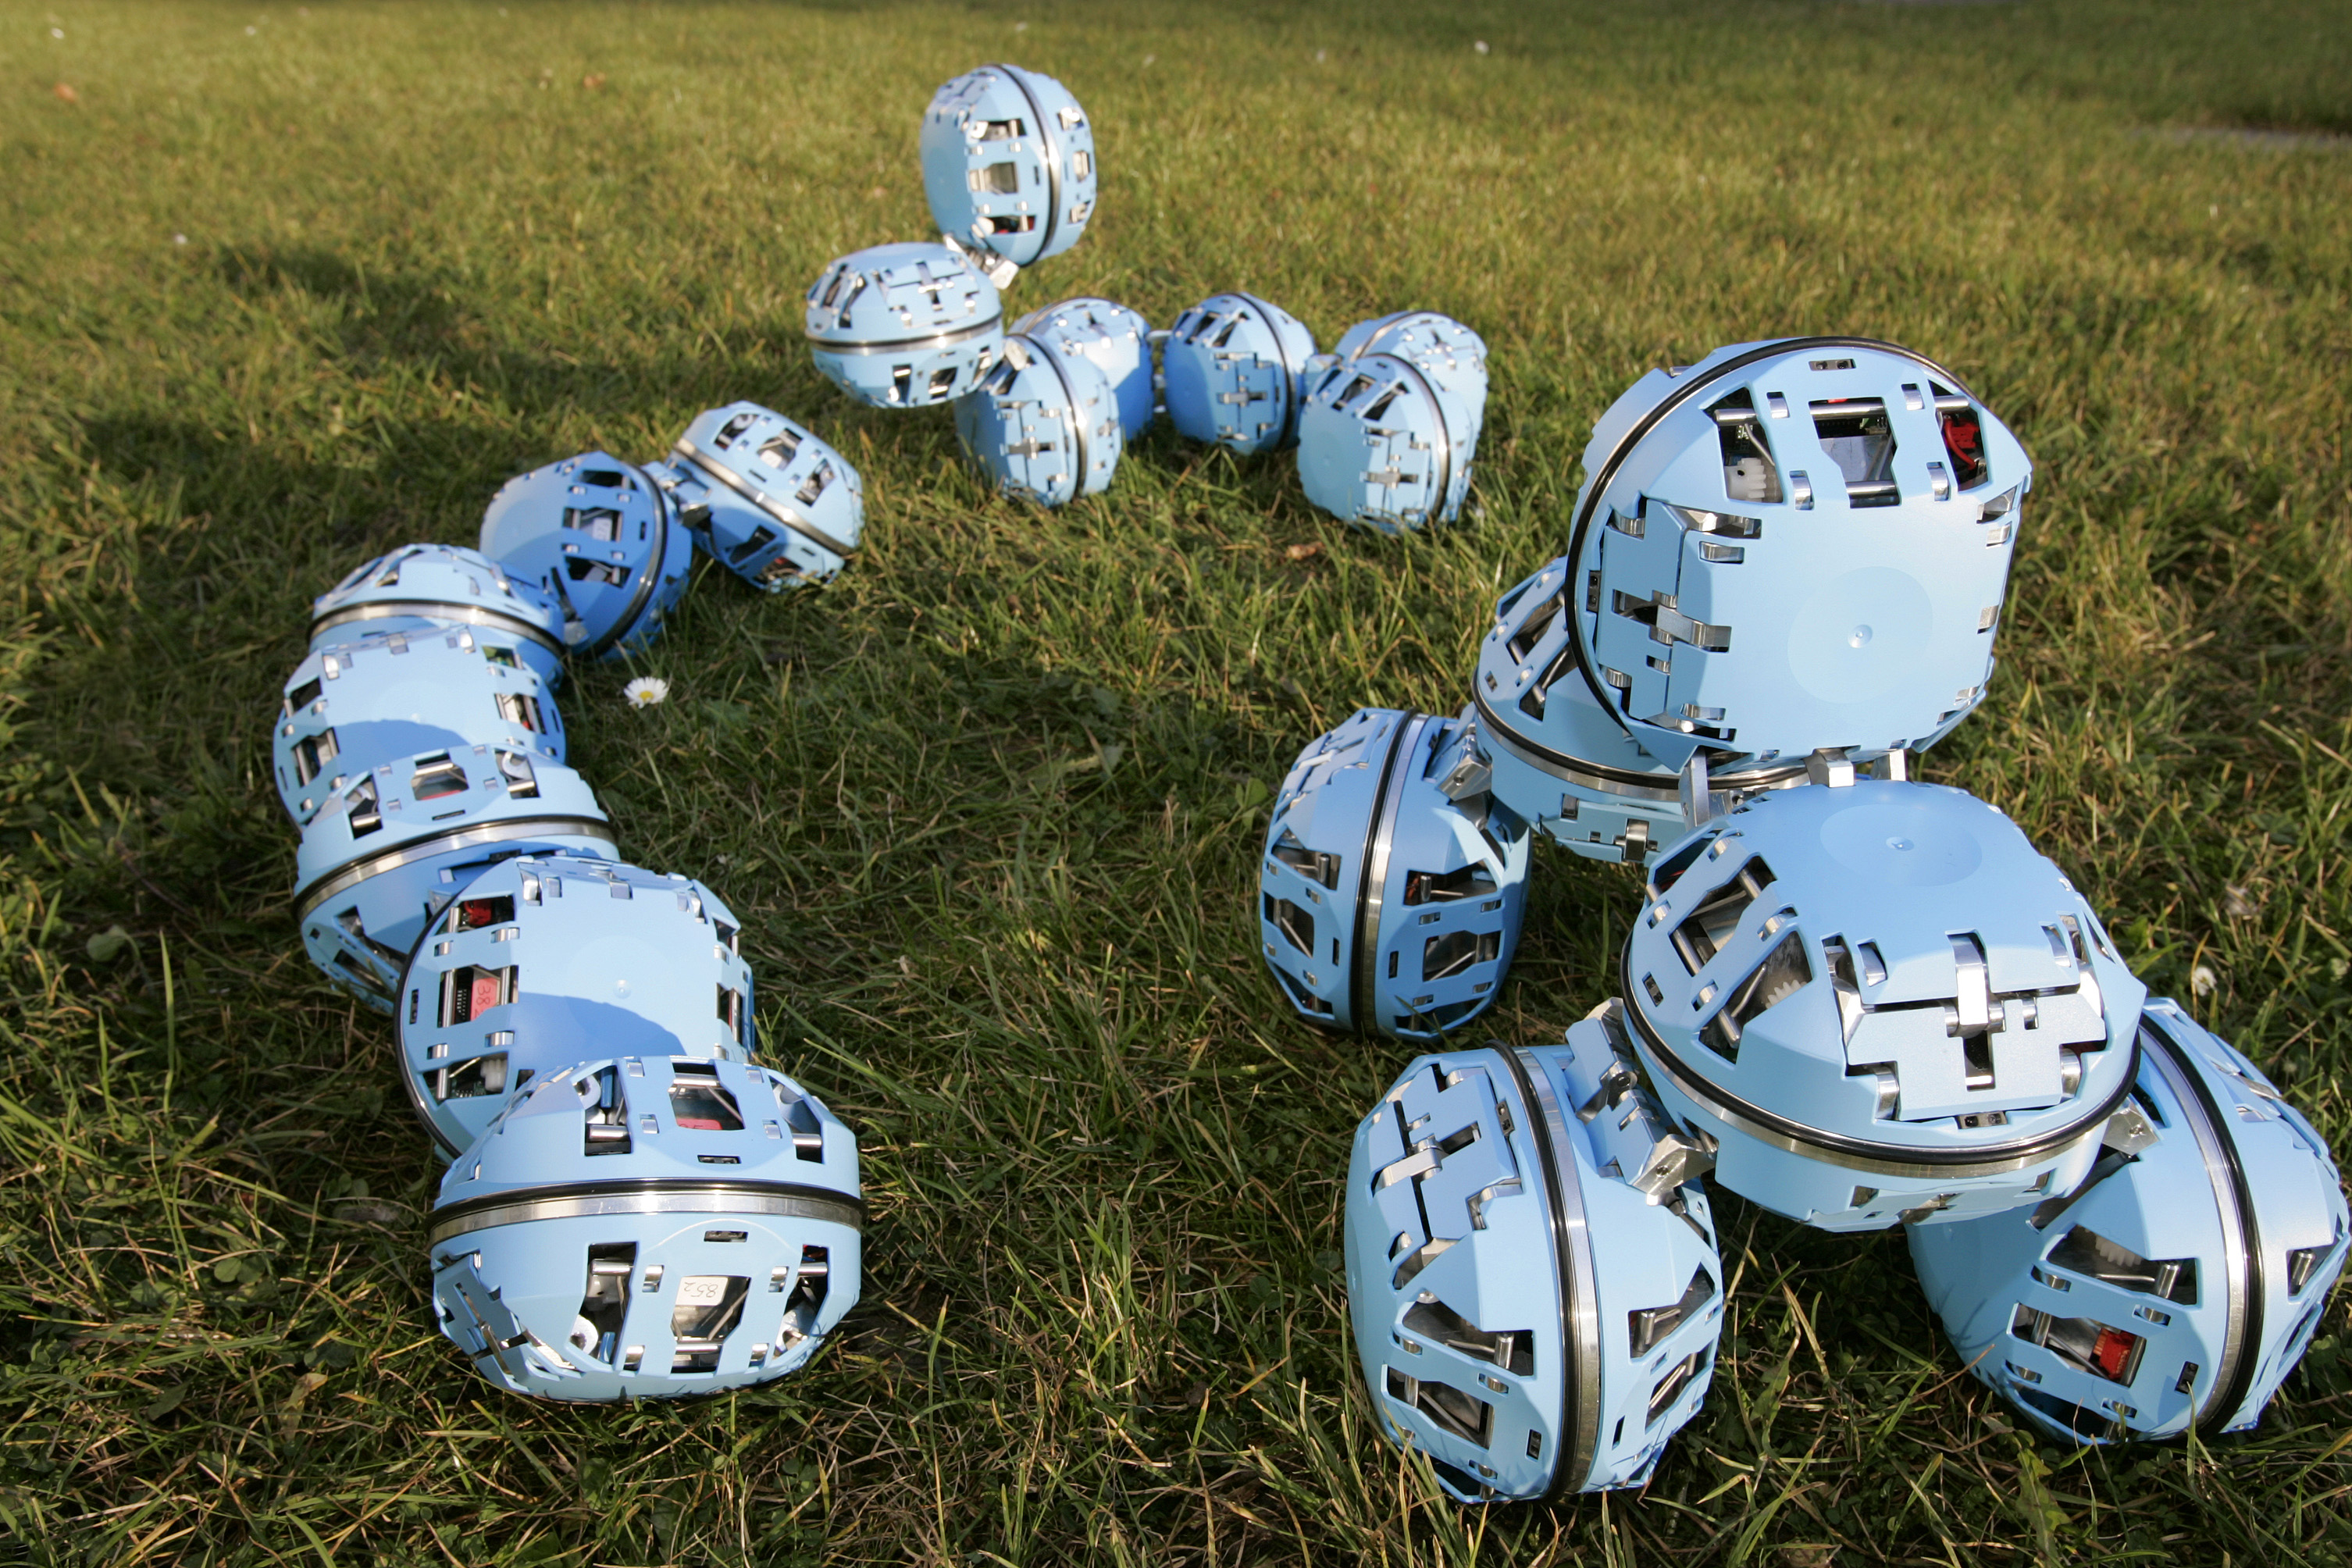
\includegraphics[width=0.45\linewidth]{ATRON.jpg}}
    \hfil
    \subfloat[][Roombots]{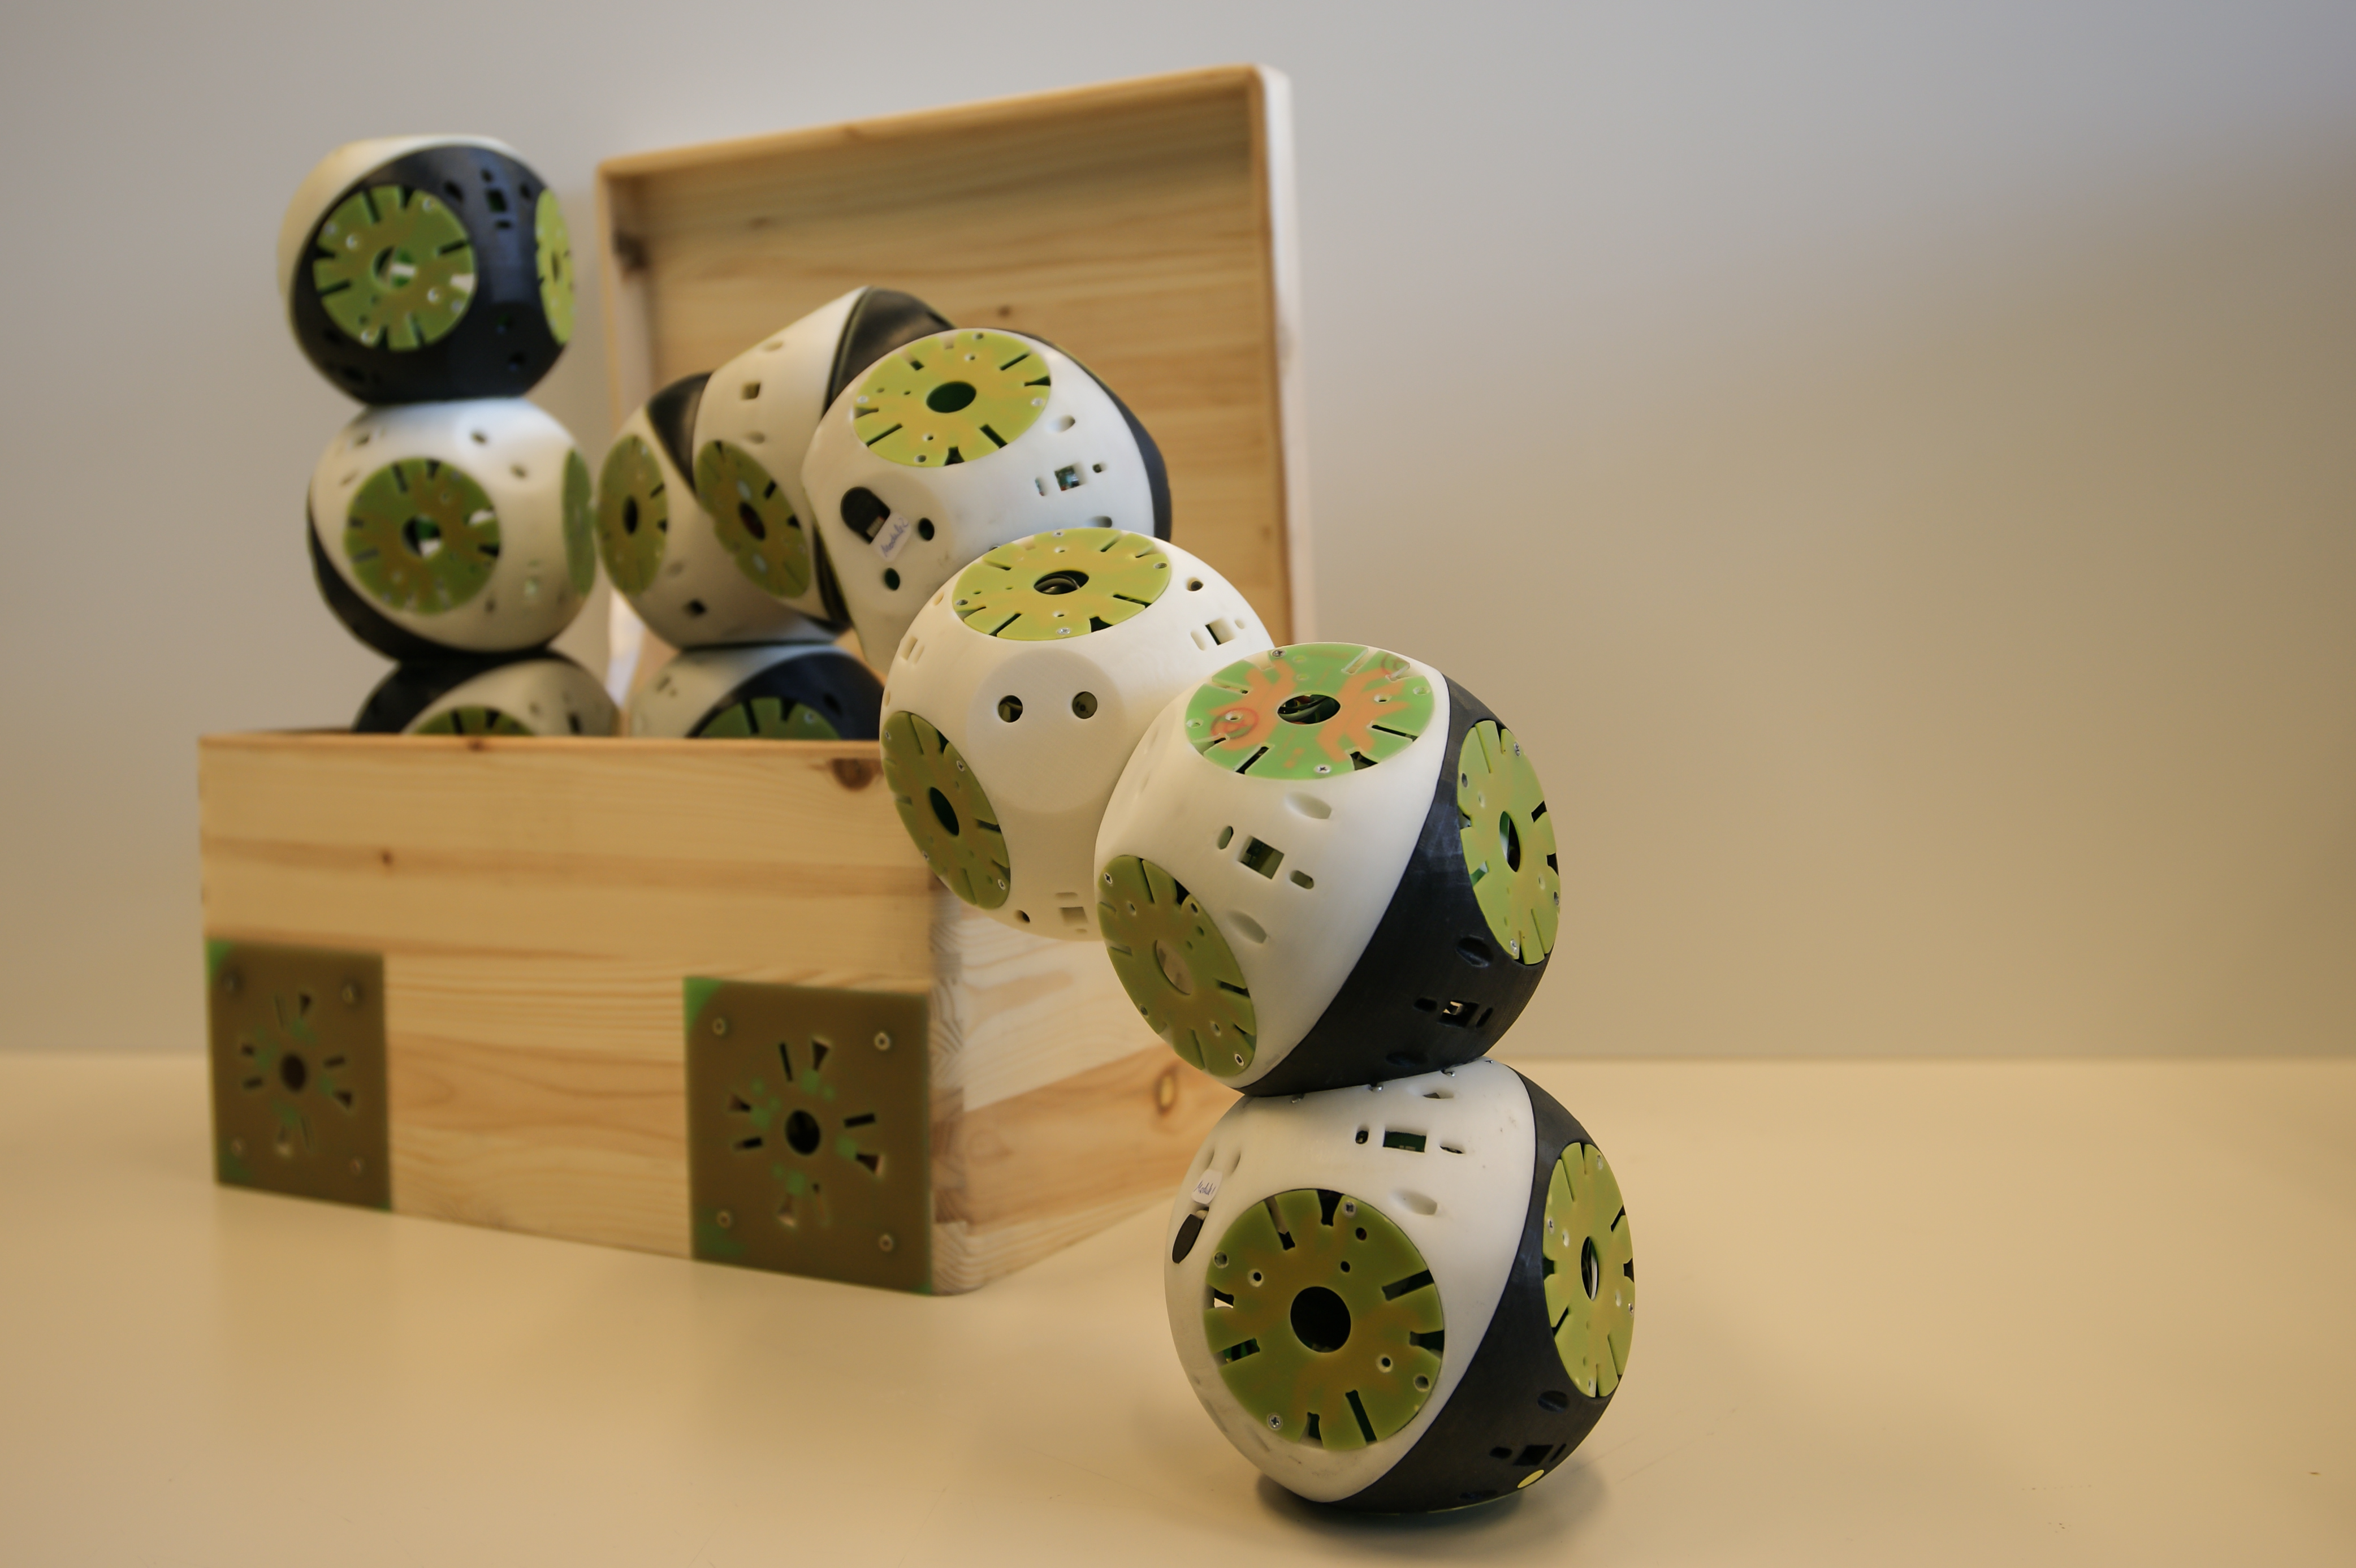
\includegraphics[width=0.45\linewidth]{roombots.jpg}}
    \caption{Modular robots}
    \label{fig:modular-robots}
\end{figure}

Actually, to our best knowledge there is only one example of modular kit allowing to really explore the role of morphology. The Locomorph project~\parencite{locomorph} offers a multi-purpose hardware kit called LocoKit~\parencite{larsen2012locokit}). This kit uses carbon-fiber rods assembled with Locokit parts (see \figurename~\ref{fig:locokit-parts}). It allows quickly creating robot and studying the impact of several morphological properties such as link length, joint stiffness or mass distribution (see \figurename~\ref{fig:locokit}). Also it permits to add spring over rods to create linear damping system and therefore add compliance to robots.
The kit is distributed for \texteuro2500 and includes the needed components to create a quadruped robot (see \figurename~\ref{fig:locokit-example}).

\begin{figure}[tb]
\centering
    \subfloat[][]{\label{fig:locokit-parts}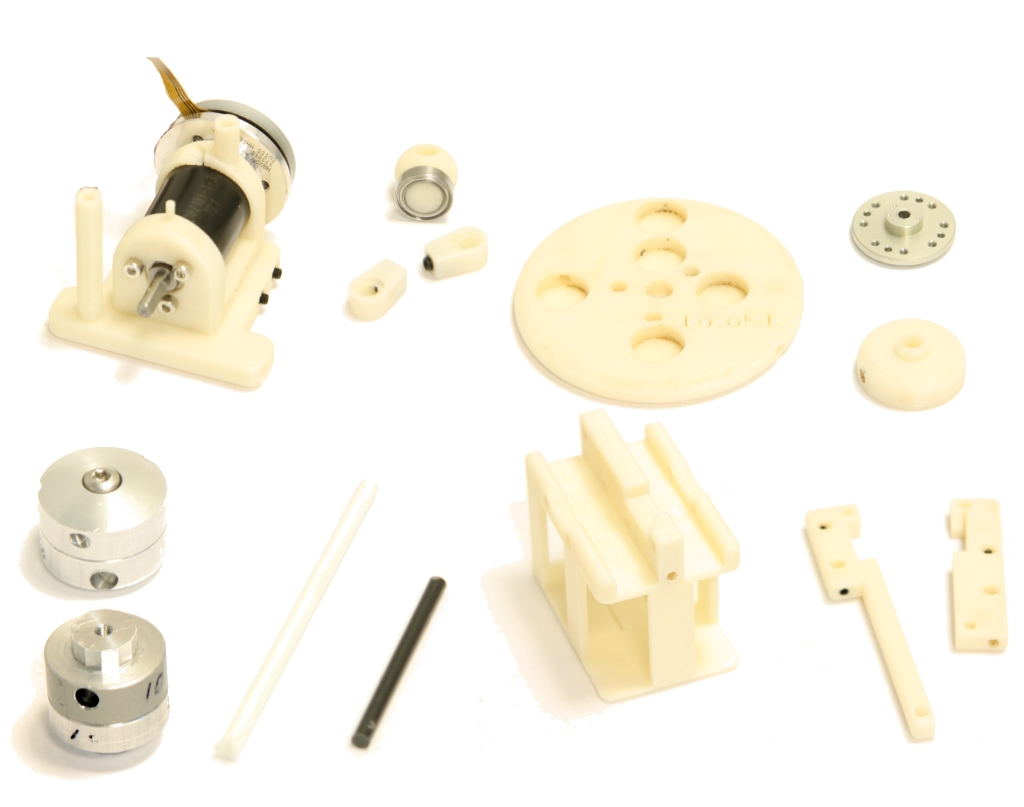
\includegraphics[height=5cm]{locokit-parts.jpg}}
    \hfil
    \subfloat[][]{\label{fig:locokit-example}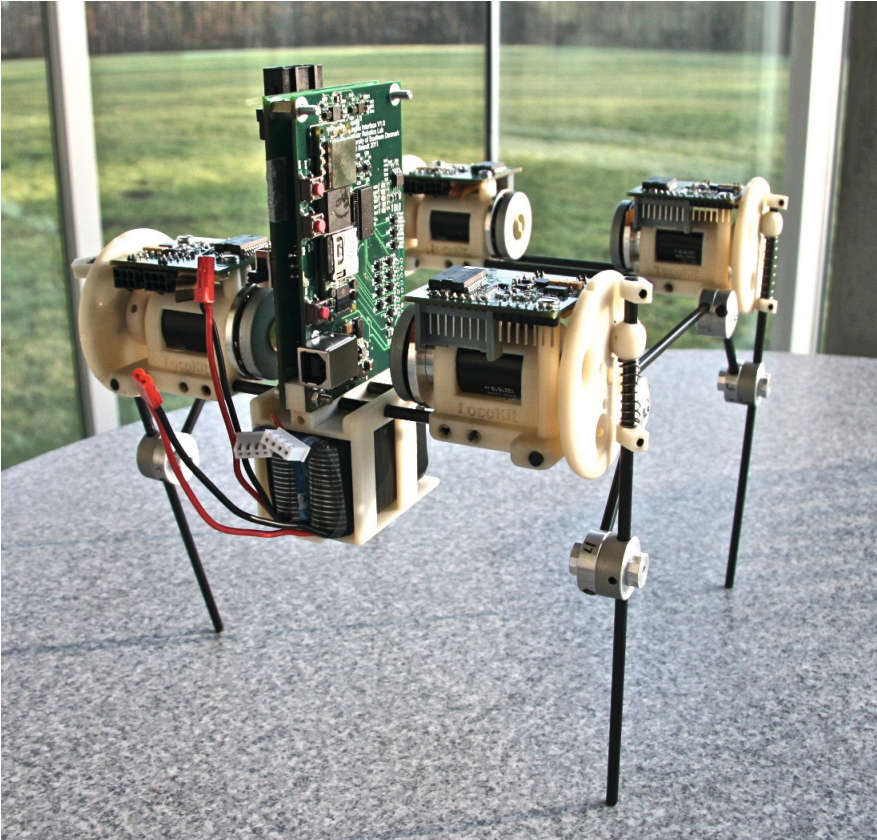
\includegraphics[height=5cm]{locokit-example.png}}
    \caption{}
    \label{fig:locokit}
\end{figure}

It appears as the only existing solution allowing to both explore the role of morphology and transfer results between laboratory. While being very interesting, it is also limited as it implies to create rods-based robot and multi-body articulation such as ones we can find in a human leg or trunk seem complicated to produce.


\section{Commercial humanoid platform} % (fold)

The robotic prototype platforms appear to share the same issue for science reproducibility. Most of them are constructed using classical manufacturing technique which make them expensive to reproduce, in addition, their have a complex morphology which make complicated the . Finally, they are in most case not open source and no material is shared allowing reproducing them easily.

The use of commercial platform can be an alternative as they are easily available, and have a constant and reproducible morphology.

\subsection{Advanced research platform} % (fold)

The two most famous humanoid robots are iCub~\parencite{metta2008icub} and HRP-2. These robots involve very advanced technologies:

ICub as an open source\footnote{The hardware design, software and documentation are released under the GPL license.} robot measuring about 100 cm high for an overall weight of 22 Kg. It has 53 degrees of freedom designed specifically for manipulation and locomotion, and powered by high-ended actuators based on harmonic drive reduction system and a brushless frameless motors~\parencite{natale2013icub}. In addition, in the majority of the cases torque is transmitted from the motors to the joints using steel tendons routed in complex ways via idle pulleys.

HRP-2 is a complete humanoid of 150 cm high for 58 kg involving 30 DoFs. It also involves high end actuators with harmonic drives and cooling systems installed in both computer and actuator drive systems to improve temperature control, yet contrary to the ICub robot, they made the choice to have the robot as stiff as possible.

Both robots involve a very complex and advanced design, which has required the work of dozens of engineers, also their production techniques make them very expensive (i.e. more than \texteuro200,000). Therefore, these robots do not permit to freely change their morphologies. Moreover, their high cost and their fragility limit the risk can take researchers to explore behaviour in the real world.



\subsection{affordable platform} % (fold)

On the other hand, there are small and affordable commercial humanoids platforms, easily accessible and easy to use such as Nao \cite{gouaillier2008nao}, Darwin Op \cite{ha2011development}, Nimbro Op \cite{schwarznimbro} or iCub \cite{metta2008icub}.

\begin{figure}[tb]
\centering
    \subfloat[][Darmin Op]{\label{fig:darwin-op}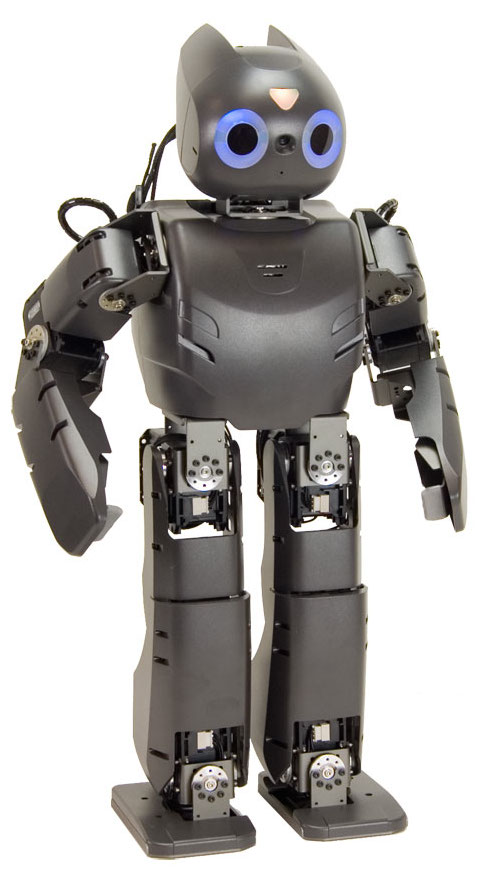
\includegraphics[height=6.5cm]{darwin_op_face.jpg}}
    \hfil
    \subfloat[][Nao]{\label{fig:Nao}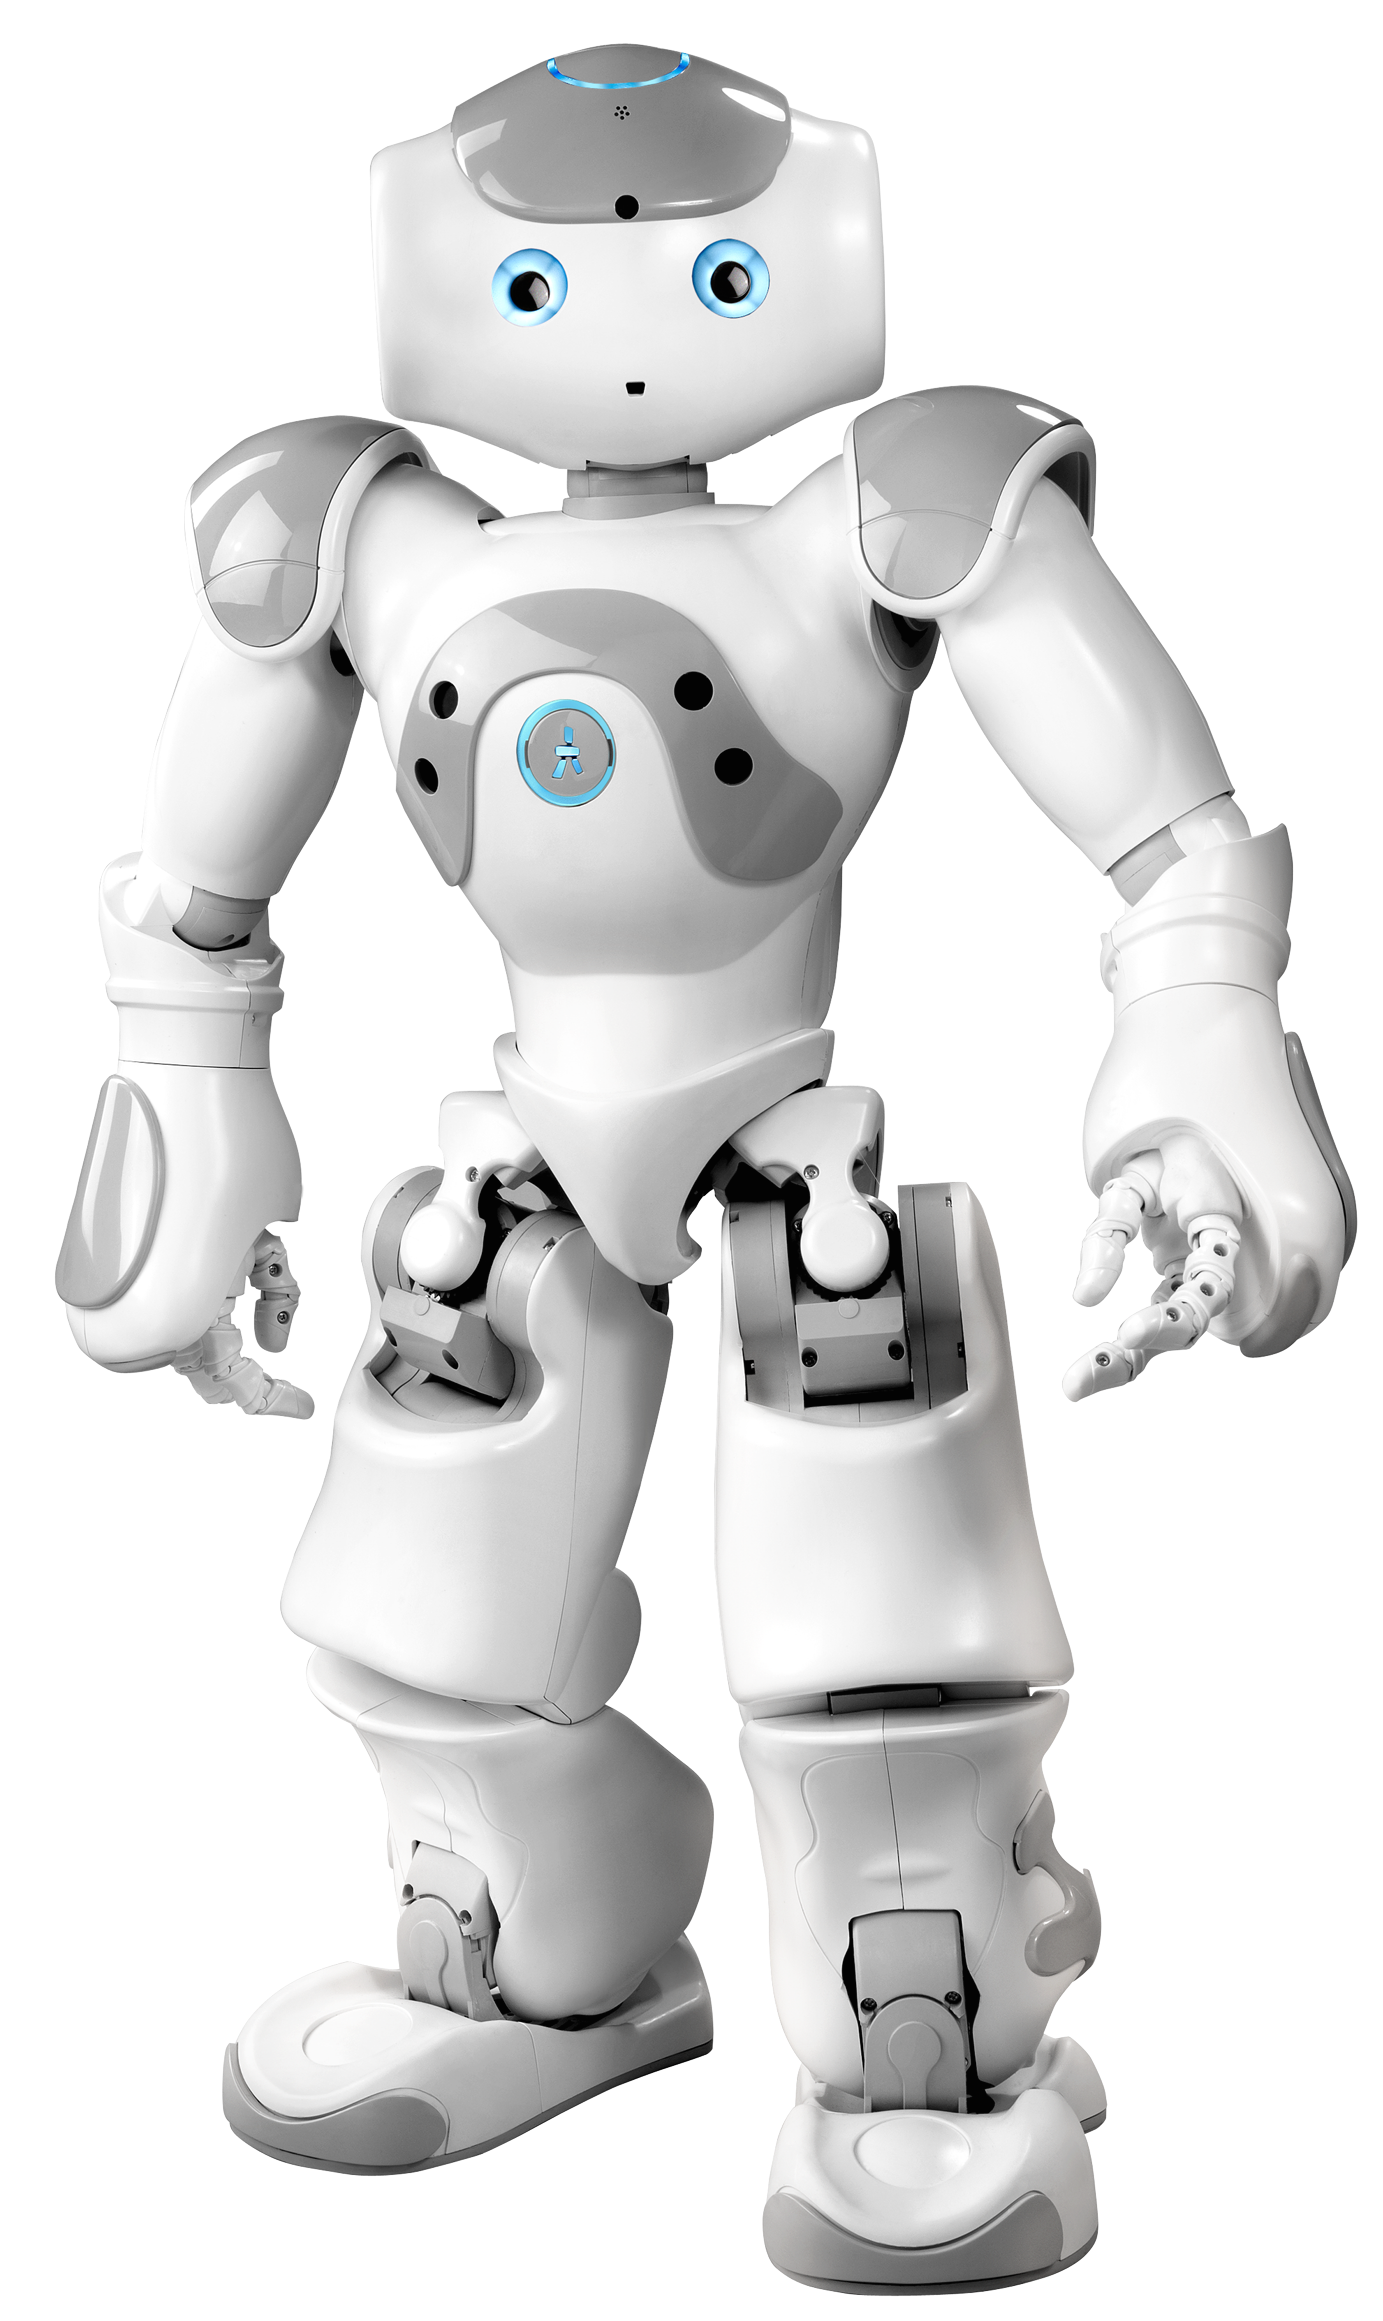
\includegraphics[height=6.5cm]{nao_face.png}}
    \hfil
    \subfloat[][Nimbro OP]{\label{fig:nimbro-op}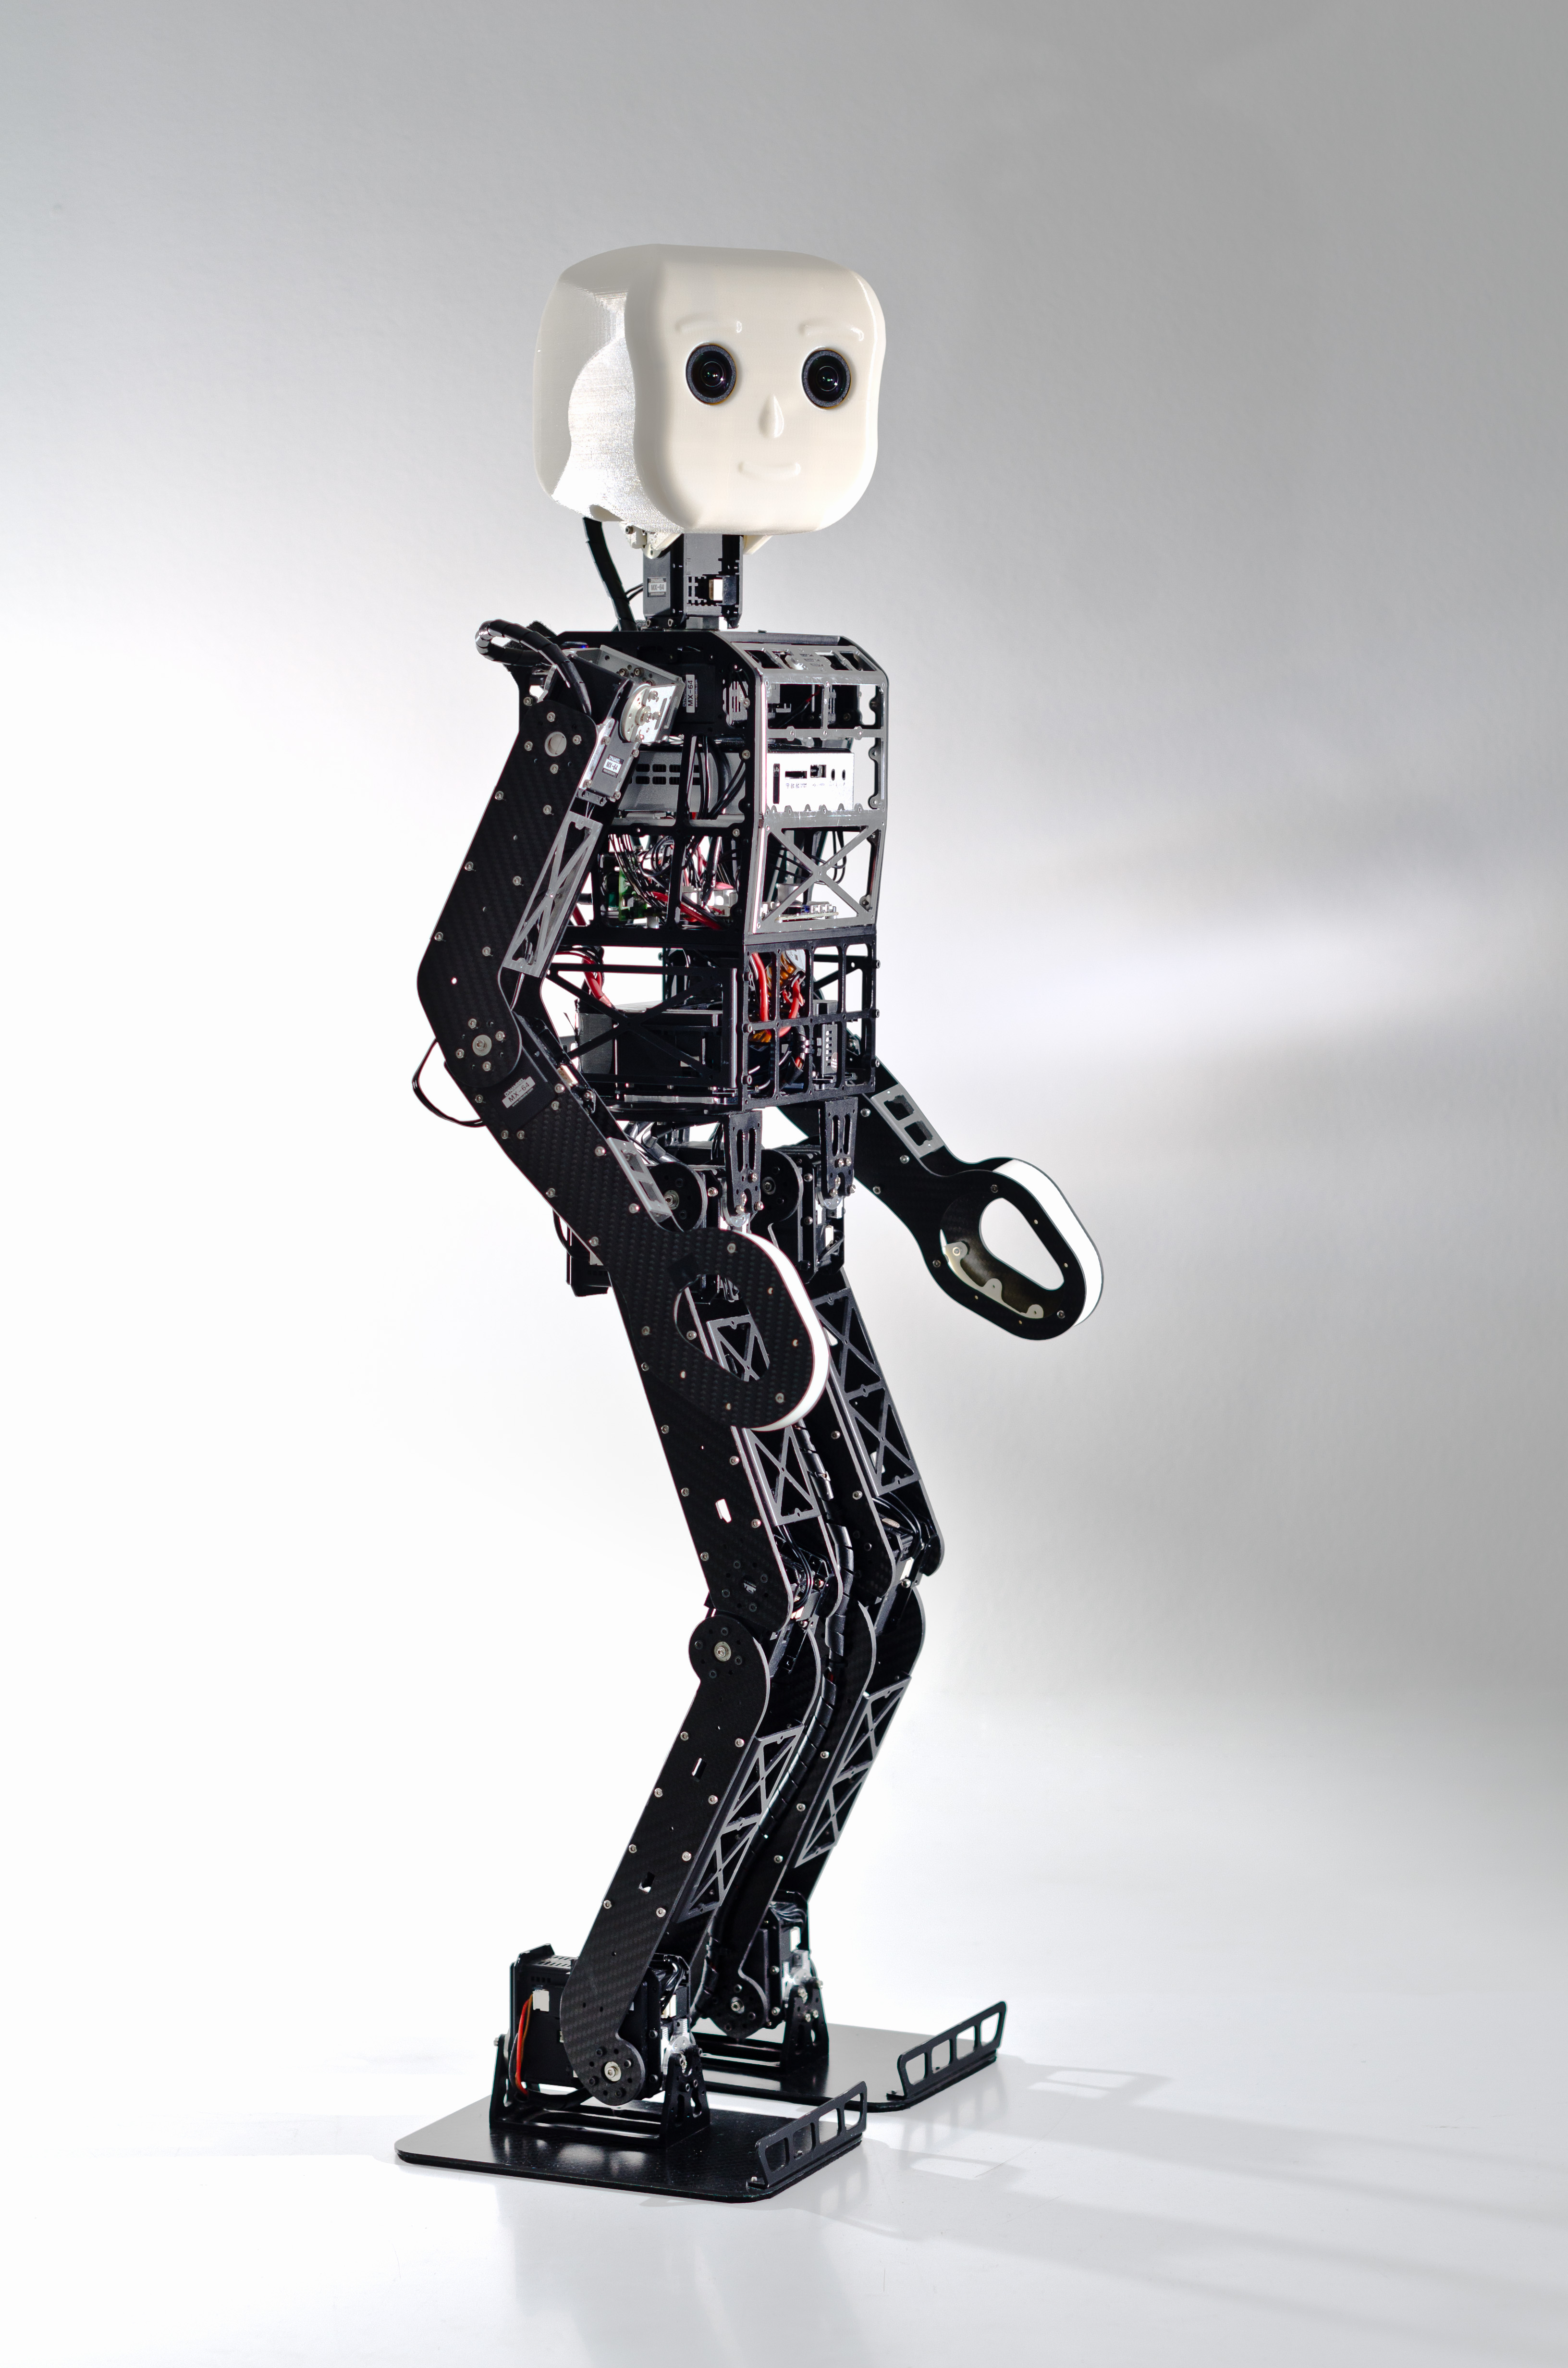
\includegraphics[height=6.5cm]{nimbro-op_1.jpg}}
    \caption{Three humanoid robots made by KumoTek (USA).}
    \label{fig:kumotek_robots}
\end{figure}


\begin{description}
    \item[DARwIn Op] is an open source humanoid research platform created by the Romela lab at Virginia tech~\parencite{ha2011development} and distributed by Robotis for about \$12,000 (see \figurename~\ref{fig:darwin-op}). It measures 45cm height, weights 2.9kg, and has 20 Dynamixel MX-28 actuators (6 for each leg, 3 for each arm, and 2 for the neck). Its mechanical structure is composed by aluminum parts.
    \item[Nao] is 55cm height, 5.2kg and 25DoFs humanoid robot with a plastic mechanical structure (ABS,PA,XCF) (see \figurename~\ref{fig:Nao}). It is a very famous robot sold by few thousands units to labs and universities. Its cost was around \texteuro12,000, but recently it was reduced by half.
    \item[Nimbro-OP] is a tall humanoid with 95cm and 6.6 kg, it has 20 powerful MX-106 and MX-64 actuators (6 per leg, 3 per arm and 2 in the neck). It costs \$20,000 and its structure is based on aluminium and carbon composite (see \figurename~\ref{fig:nimbro-op}).
\end{description}

Yet, they provide a "traditional" morphology (e.g. limited compliance, rigid torso, big feet, over actuation) not really adapted to explore the interesting morphological properties we showed in the chapter~\ref{cha:morphology-review}. Also as they use classic manufacturing techniques such as metal milling and plastic casting, the modification of their morphologies is made difficult.

\section{Conclusion}

In the previous chapter, we presented several work showing the importance of the robot morphology and the need to continue the research in this domain. As we explained in section~\ref{sec:platform-introduction}, this research requires to have real robotic platform to be explored.

There are many robotic platform, we could have a more exhaustive description, yet the main objective of this review was two show an overview of the landscape of possibility with the current robotic platform. In particular that we have on one hand, some prototype robotic platforms designed for specifically to explore an aspect of robotic morphology but which design methodology strongly limit their reproduction in the robotics community mainly because their are not open source and produced with expensive techniques.
And on the other hand, commercial robots that are easily accessible so the results should be reproducible from one lab to another. Yet their design method involved also classical production techniques, therefore modifying their morphology would be too expensive and time consuming.

Finally, the current research practices in the Robotics field limit the diffusion and the impact of contributions.
Indeed, in most cases, there is no material associated with a published paper.
Meaning, only the theory is shared with the community but not the actual framework allowing reproducing the results.

In the next chapter, we will present novel production techniques and diffusion fashion, which can solve both problem considering exploring the role of morphology and reproducibility between research labs.






